%%%%%%%%%%%%%%%%%%%%%%%%%%%%%%%%%%%%%%%%%%%%%%
%%
%%    D e s c r i p t i o n    o f     t h e      O b s e r v a t i o n s  : 
%%
%%%%%%%%%%%%%%%%%%%%%%%%%%%%%%%%%%%%%%%%%%%%%%
\smallskip
\smallskip
\noindent
Sample is given in Figure 2. There are 
11 QSOs with confirmed spectroscopic redshifts, with redshift range $5.0<z<6.7$ and
strong, SNR$\geq 5$ WISE detections in the W3 12$\mu$m band.

\smallskip
\smallskip
\noindent
Things to think about::\\
NIRSpec vs. NIRISS?\\
NIRSpec since it has the higher resolution modes

\smallskip
\smallskip
\noindent
Things to think about::\\
NIRSpec IFU vs.  NIRSpec fixed slits (FS) ?? \\
Both have $\approx$the same wavelength coverage. Need to run ETC. 


\smallskip
\smallskip
\noindent
Our targets are well spaced in R.A. and Decl.


\hspace{-7.5cm}
\begin{figure}[h]
  \begin{center}
    \hspace{-0.5cm}
%    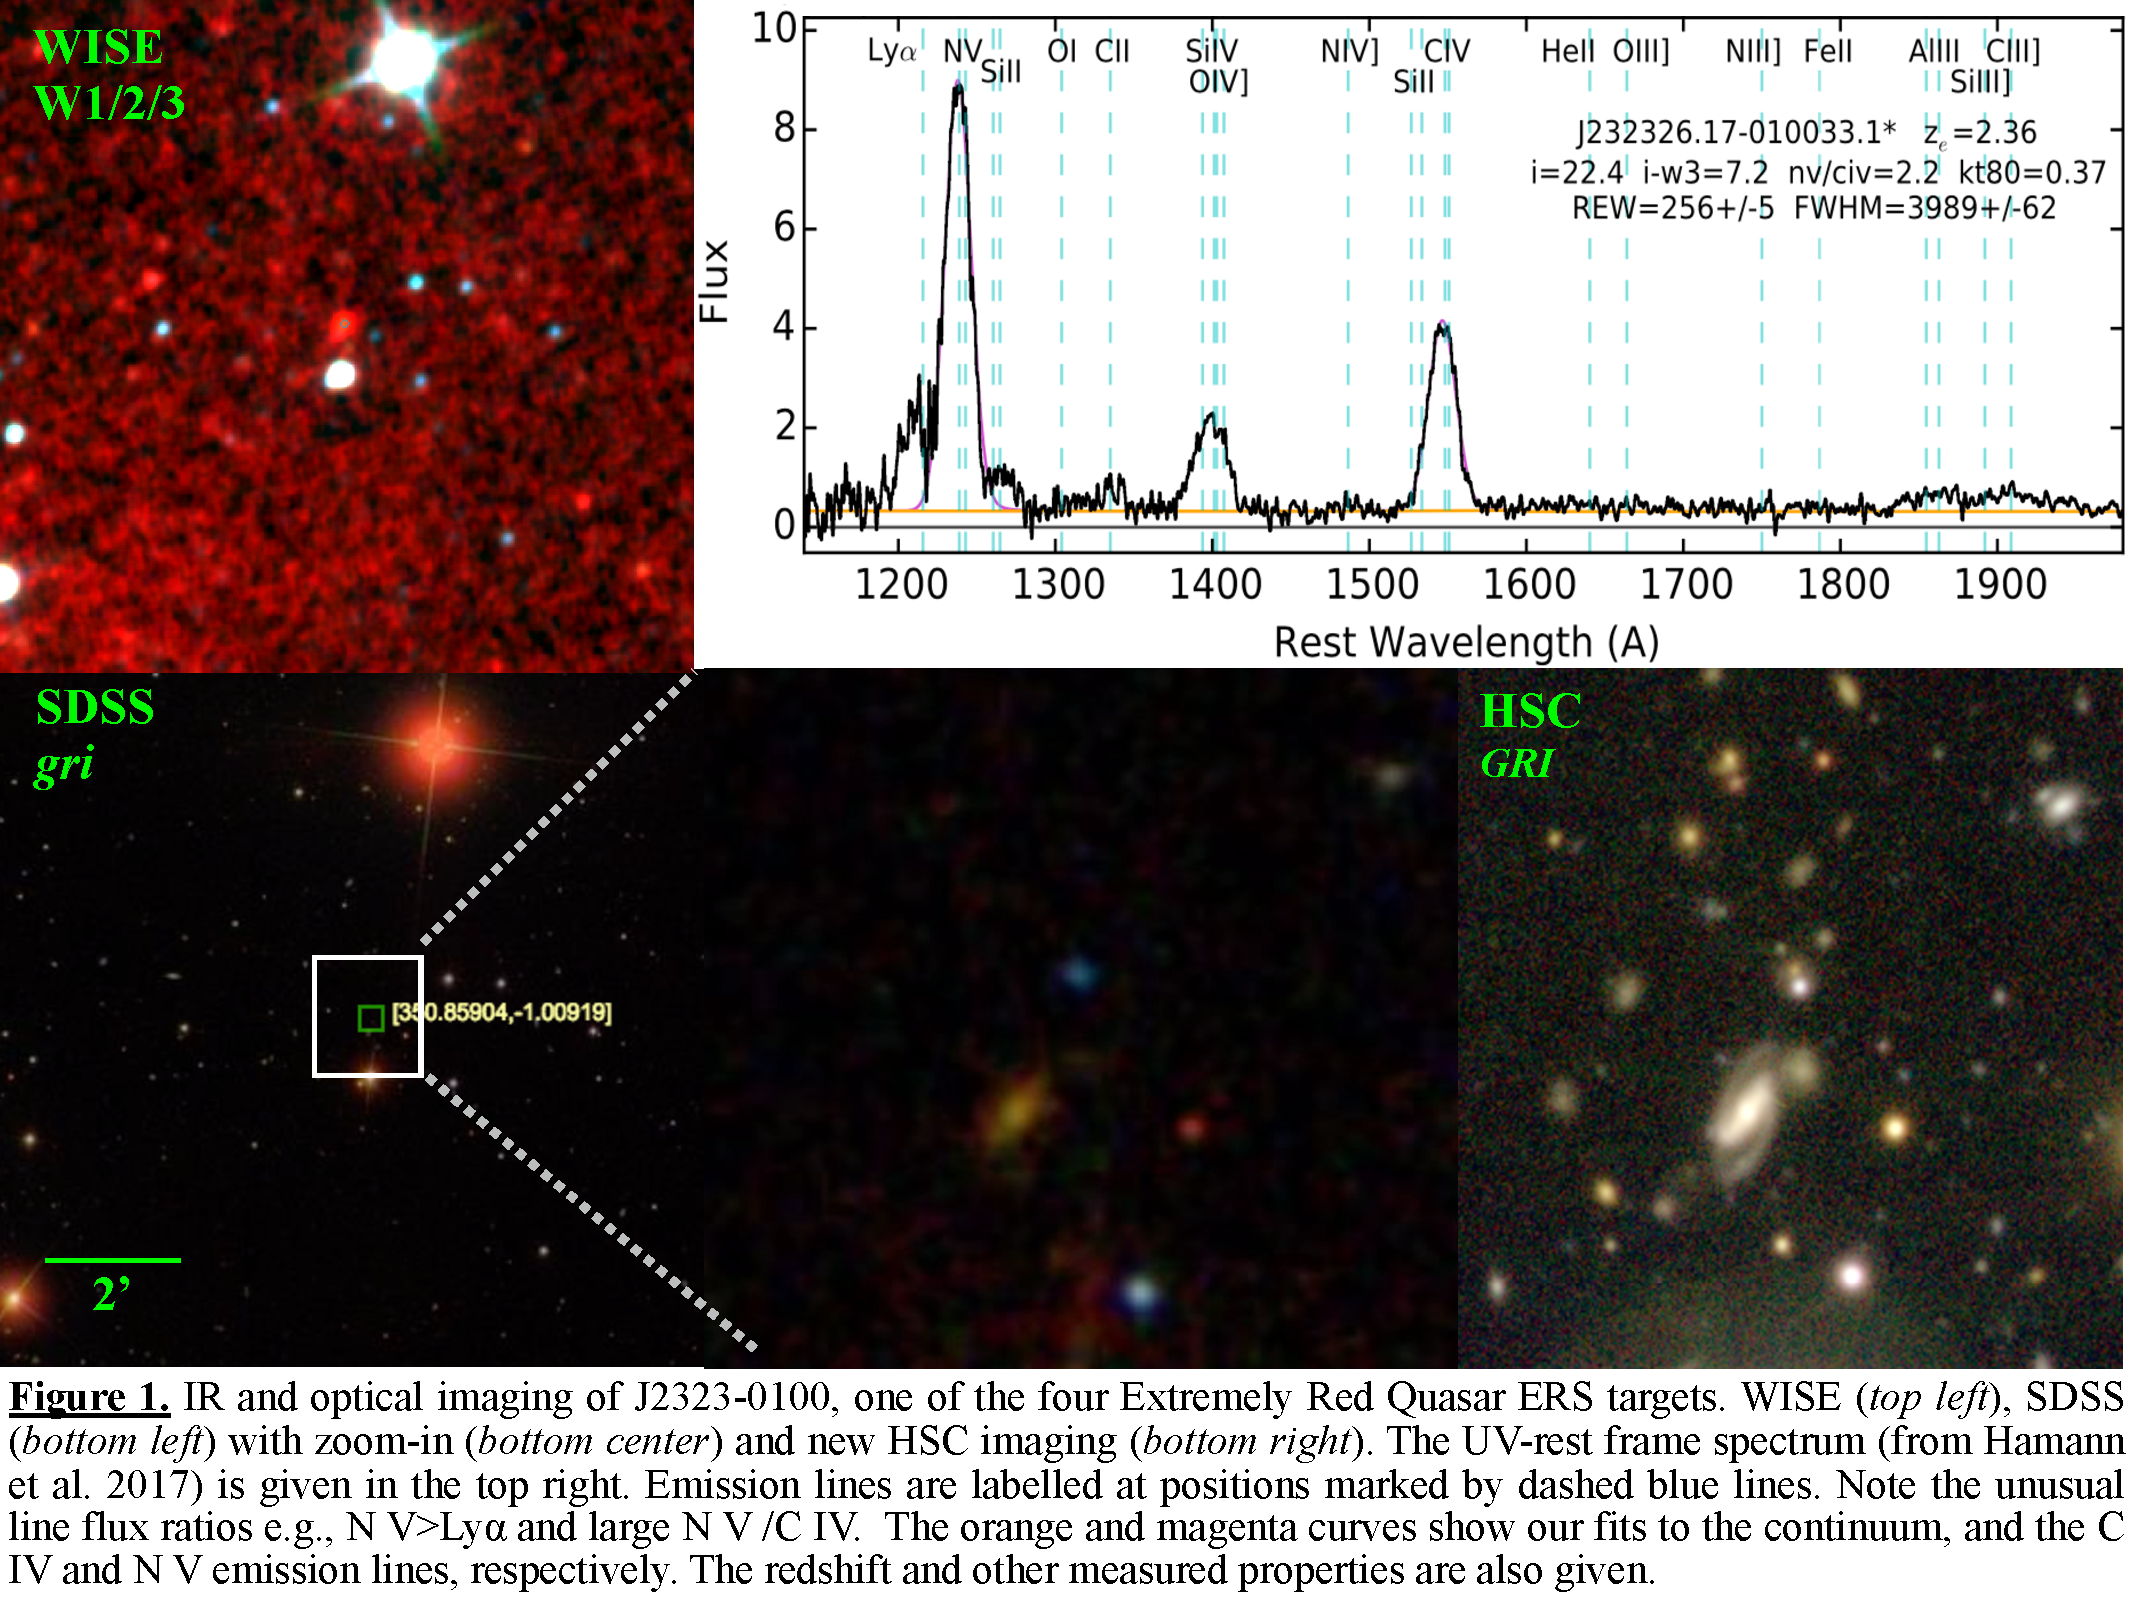
\includegraphics[]{WISE_SDSSzoomHSC_ERQ-image_v2.pdf}
    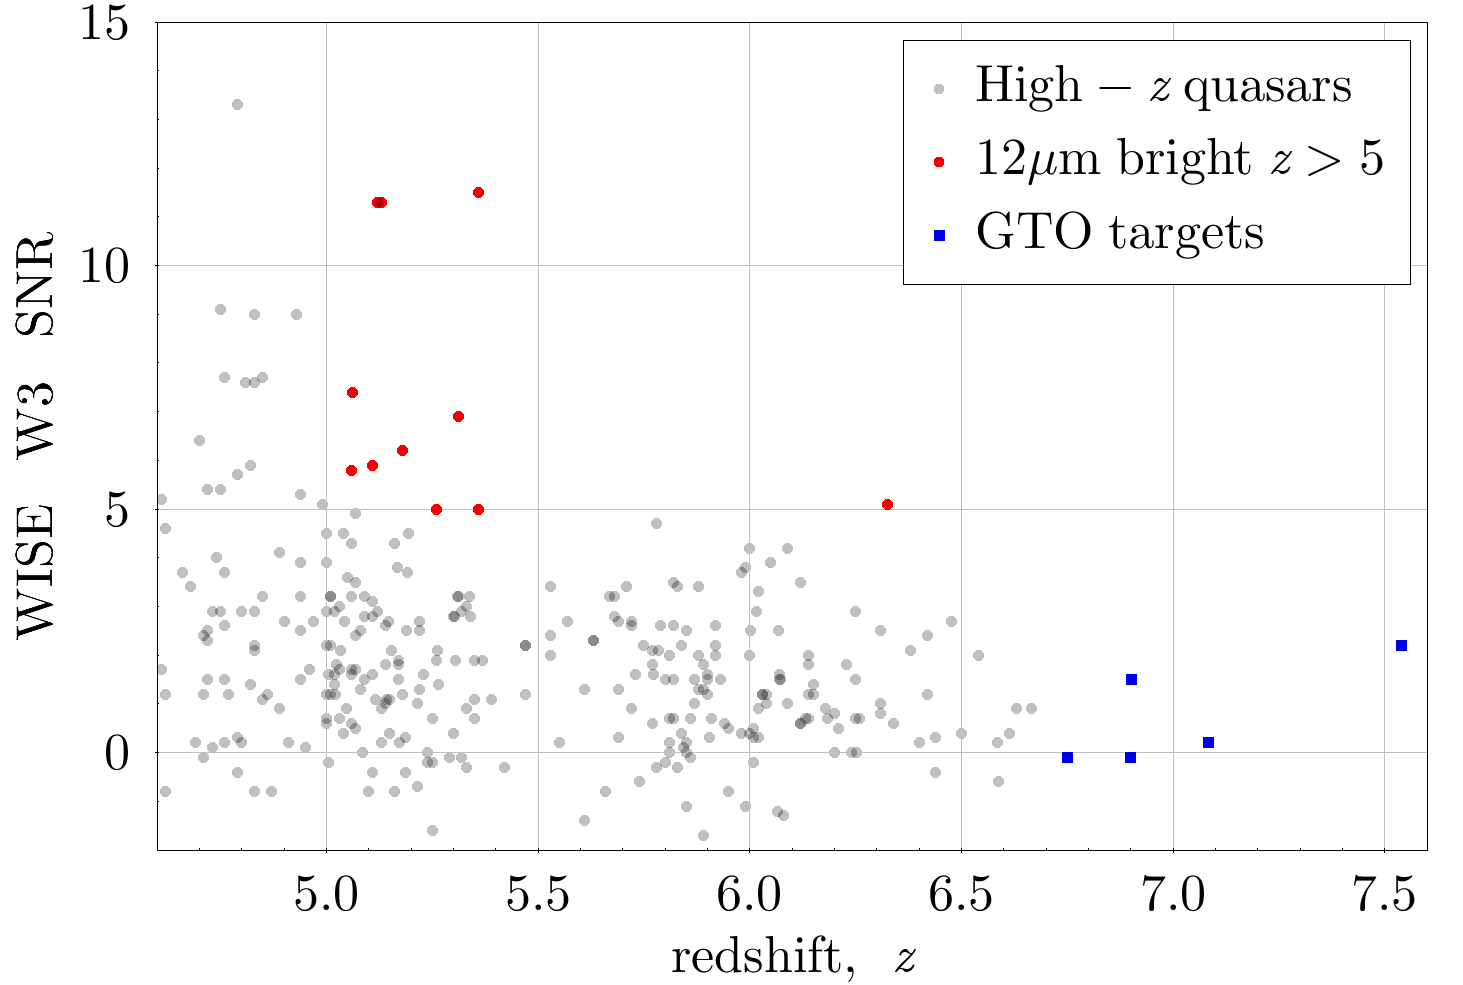
\includegraphics[height=12.0cm,width=16.0cm]{../Figures/VHzQ_WISE_W3SNR_vs_redshift.png}
    \vspace{-10pt}
\caption{The WISE W3 SNR values for all spectroscopically confirmed $z\geq5$ quasars. 
Our sample are the red circles; the GTO reserved targets are the blue squares.}
    \label{figtest-fig}
  \end{center}
\end{figure}



